% Options for packages loaded elsewhere
\PassOptionsToPackage{unicode}{hyperref}
\PassOptionsToPackage{hyphens}{url}
%
\documentclass[
  10pt,
  ignorenonframetext,
]{beamer}
\usepackage{pgfpages}
\setbeamertemplate{caption}[numbered]
\setbeamertemplate{caption label separator}{: }
\setbeamercolor{caption name}{fg=normal text.fg}
\beamertemplatenavigationsymbolsempty
% Prevent slide breaks in the middle of a paragraph
\widowpenalties 1 10000
\raggedbottom
\setbeamertemplate{part page}{
  \centering
  \begin{beamercolorbox}[sep=16pt,center]{part title}
    \usebeamerfont{part title}\insertpart\par
  \end{beamercolorbox}
}
\setbeamertemplate{section page}{
  \centering
  \begin{beamercolorbox}[sep=12pt,center]{part title}
    \usebeamerfont{section title}\insertsection\par
  \end{beamercolorbox}
}
\setbeamertemplate{subsection page}{
  \centering
  \begin{beamercolorbox}[sep=8pt,center]{part title}
    \usebeamerfont{subsection title}\insertsubsection\par
  \end{beamercolorbox}
}
\AtBeginPart{
  \frame{\partpage}
}
\AtBeginSection{
  \ifbibliography
  \else
    \frame{\sectionpage}
  \fi
}
\AtBeginSubsection{
  \frame{\subsectionpage}
}
\usepackage{amsmath,amssymb}
\usepackage{lmodern}
\usepackage{setspace}
\usepackage{iftex}
\ifPDFTeX
  \usepackage[T1]{fontenc}
  \usepackage[utf8]{inputenc}
  \usepackage{textcomp} % provide euro and other symbols
\else % if luatex or xetex
  \usepackage{unicode-math}
  \defaultfontfeatures{Scale=MatchLowercase}
  \defaultfontfeatures[\rmfamily]{Ligatures=TeX,Scale=1}
\fi
% Use upquote if available, for straight quotes in verbatim environments
\IfFileExists{upquote.sty}{\usepackage{upquote}}{}
\IfFileExists{microtype.sty}{% use microtype if available
  \usepackage[]{microtype}
  \UseMicrotypeSet[protrusion]{basicmath} % disable protrusion for tt fonts
}{}
\makeatletter
\@ifundefined{KOMAClassName}{% if non-KOMA class
  \IfFileExists{parskip.sty}{%
    \usepackage{parskip}
  }{% else
    \setlength{\parindent}{0pt}
    \setlength{\parskip}{6pt plus 2pt minus 1pt}}
}{% if KOMA class
  \KOMAoptions{parskip=half}}
\makeatother
\usepackage{xcolor}
\geometry{left = 1cm, right = 0.5cm, top = 0.5cm, bottom = 0.5cm}
\newif\ifbibliography
\setlength{\emergencystretch}{3em} % prevent overfull lines
\providecommand{\tightlist}{%
  \setlength{\itemsep}{0pt}\setlength{\parskip}{0pt}}
\setcounter{secnumdepth}{-\maxdimen} % remove section numbering
\titlegraphic{
\includegraphics[scale=0.05]{pictures/GlaLogo.pdf}}
\usepackage{float}
\usepackage{booktabs}
\usepackage{array}
\usepackage{longtable}
\useinnertheme{rectangles}
\setbeamertemplate{itemize subitem}{\scriptsize$\diamond$}
\definecolor{blue}{RGB}{0,114,178}
\definecolor{red}{RGB}{213,94,0}
\definecolor{yellow}{RGB}{240,228,66}
\definecolor{green}{RGB}{0,158,115}
\ifLuaTeX
  \usepackage{selnolig}  % disable illegal ligatures
\fi
\IfFileExists{bookmark.sty}{\usepackage{bookmark}}{\usepackage{hyperref}}
\IfFileExists{xurl.sty}{\usepackage{xurl}}{} % add URL line breaks if available
\urlstyle{same} % disable monospaced font for URLs
\hypersetup{
  pdftitle={Introductory Statistics for Economics},
  pdfauthor={Duong Trinh},
  hidelinks,
  pdfcreator={LaTeX via pandoc}}

\title{Introductory Statistics for Economics}
\subtitle{ECON1013: LAB 1}
\author{Duong Trinh}
\date{Jan 2024}
\institute{University of Glasgow}

\begin{document}
\frame{\titlepage}

\setstretch{1.5}
\begin{frame}{Intro}
\protect\hypertarget{intro}{}
\begin{itemize}
\tightlist
\item
  Duong Trinh

  \begin{itemize}
  \tightlist
  \item
    PhD Student in Economics (Bayesian Microeconometrics)
  \item
    Email: \underline{Duong.Trinh@glasgow.ac.uk}
  \end{itemize}
\end{itemize}

\vspace{3mm}

\begin{itemize}
\tightlist
\item
  ECON1013-LB04

  \begin{itemize}
  \tightlist
  \item
    Monday 1-2 pm
  \item
    3 sessions (29-Jan, 12-Feb, 26-Feb)
  \end{itemize}
\item
  ECON1013-LB05

  \begin{itemize}
  \tightlist
  \item
    Tuesday 12-1 pm
  \item
    3 sessions (30-Jan, 13-Feb, 27-Feb)
  \end{itemize}
\item
  ECON1013-LB06

  \begin{itemize}
  \tightlist
  \item
    Tuesday 1-2 pm
  \item
    3 sessions (30-Jan, 13-Feb, 27-Feb)
  \end{itemize}
\end{itemize}

\vspace{3mm}
\end{frame}

\begin{frame}{Record Attendance}
\protect\hypertarget{record-attendance}{}
\end{frame}

\begin{frame}{Setup}
\protect\hypertarget{setup}{}
\begin{itemize}
\item
  Step 1: Download Lab materials from \textbf{Moodle} page
  \(\rightarrow\) Extract the folder in PC.
\item
  Step 2: Log in \textbf{Microsoft onedrive} using your student account
  \textcolor{blue}{https://onedrive.live.com/login/} and upload the
  folder above.
\item
  Step 3: Launch the \textbf{Excel} online
  \textcolor{blue}{https://www.office.com/launch/excel?auth=2}, which we
  will use for all lab sessions.
\end{itemize}
\end{frame}

\hypertarget{preliminaries}{%
\section{PRELIMINARIES}\label{preliminaries}}

\begin{frame}{The Excel Interface}
\protect\hypertarget{the-excel-interface}{}
\begin{block}{Ribbon}
\protect\hypertarget{ribbon}{}
\end{block}

\begin{block}{Workbook and Worksheets}
\protect\hypertarget{workbook-and-worksheets}{}
\end{block}

\begin{block}{Rows, Columns, and Cells}
\protect\hypertarget{rows-columns-and-cells}{}
\end{block}
\end{frame}

\begin{frame}{The Excel Interface}
\protect\hypertarget{the-excel-interface-1}{}
\begin{block}{Ribbon}
\protect\hypertarget{ribbon-1}{}
\begin{center}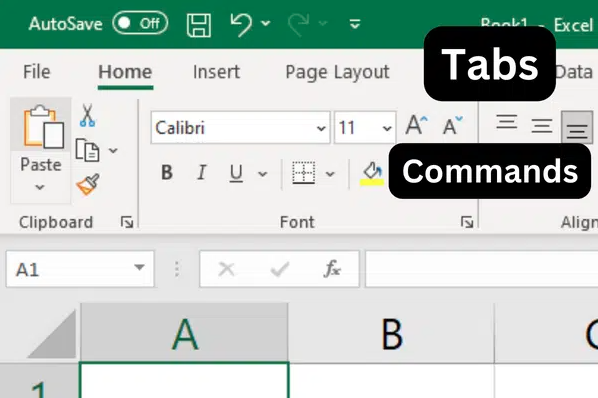
\includegraphics[width=0.5\linewidth]{pictures/Excel-ribbon} \end{center}

\begin{itemize}
\item
  To show or hide the ribbon commands, press \textbf{Ctrl-F1}.
\item
  If you can't remember the location of a command, you can always use
  the search bar on the ribbon to find it.
\end{itemize}
\end{block}
\end{frame}

\begin{frame}{The Excel Interface}
\protect\hypertarget{the-excel-interface-2}{}
\begin{block}{Workbook and Worksheets}
\protect\hypertarget{workbook-and-worksheets-1}{}
\begin{center}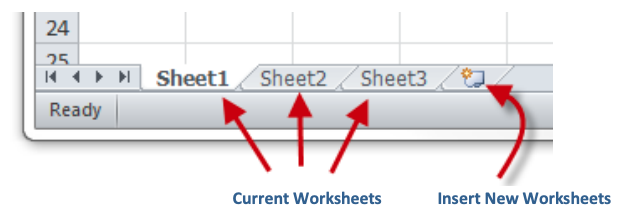
\includegraphics[width=0.5\linewidth]{pictures/Excel-worksheets} \end{center}

\begin{quote}
A workbook is an Excel file that contains one or more worksheets.
Worksheets are where you organize and process your data.
\end{quote}

\begin{itemize}
\item
  To navigate through your worksheets using keyboard shortcuts:

  \begin{itemize}
  \item
    Press \textbf{Ctrl + Page Up} to move to the next sheet.
  \item
    Press \textbf{Ctrl + Page Down} to move to the previous sheet.
  \end{itemize}
\end{itemize}
\end{block}
\end{frame}

\begin{frame}{The Excel Interface}
\protect\hypertarget{the-excel-interface-3}{}
\begin{block}{Rows, Columns, and Cells}
\protect\hypertarget{rows-columns-and-cells-1}{}
\begin{center}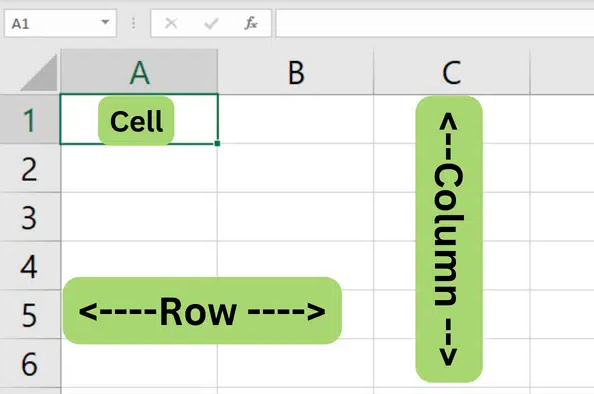
\includegraphics[width=0.5\linewidth]{pictures/Excel-cells} \end{center}

\begin{itemize}
\item
  To navigate within a worksheet, use the arrow keys to move up, down,
  left, or right.
\item
  To select a range of cells, click and drag with your mouse or hold the
  Shift key while using the arrow keys.
\item
  To quickly select the entire row or column, click on the row number or
  column letter.
\end{itemize}
\end{block}
\end{frame}

\begin{frame}{Excel Formulas and Functions}
\protect\hypertarget{excel-formulas-and-functions}{}
\begin{block}{Excel Formulas}
\protect\hypertarget{excel-formulas}{}
\end{block}

\begin{block}{Cell Referencing}
\protect\hypertarget{cell-referencing}{}
\end{block}

\begin{block}{Excel Math Functions}
\protect\hypertarget{excel-math-functions}{}
\end{block}
\end{frame}

\begin{frame}[fragile]{Excel Formulas and Functions}
\protect\hypertarget{excel-formulas-and-functions-1}{}
\begin{block}{Excel Formulas}
\protect\hypertarget{excel-formulas-1}{}
\vspace{3mm}

\begin{quote}
Formulas in Excel are used to perform calculations and manipulate data
with built-in functions.
\end{quote}

\begin{itemize}
\item
  To create a formula, start with an equal sign (\(\textbf{=}\))
  followed by a combination of numbers, cell references, and
  mathematical operators.
\item
  Here is an example that adds the values in the range \texttt{A1} to
  \texttt{A5}: \(\textbf{\texttt{=SUM(A1:A5)}}\).
\end{itemize}
\end{block}
\end{frame}

\begin{frame}{Excel Formulas and Functions}
\protect\hypertarget{excel-formulas-and-functions-2}{}
\begin{block}{Cell Referencing}
\protect\hypertarget{cell-referencing-1}{}
\begin{quote}
Cell referencing is a way to point to a specific cell or range of cells
in a formula. There are two types of cell references: absolute and
relative.
\end{quote}

\begin{itemize}
\item
  \textcolor{green}{\textbf{Absolute}}: refers to a specific cell or
  range and keeps the same reference even when the formula is copied. It
  uses a dollar sign (\(\texttt{\$}\)) to denote absolute referencing,
  like \(\texttt{\$A\$1}\).
\item
  \textcolor{green}{\textbf{Relative}}: A relative reference changes
  when the formula is copied to another cell or range, adjusting the
  reference based on the new location.
\end{itemize}
\end{block}
\end{frame}

\begin{frame}{Excel Formulas and Functions}
\protect\hypertarget{excel-formulas-and-functions-3}{}
\begin{block}{Excel Math Functions}
\protect\hypertarget{excel-math-functions-1}{}
Here are some commonly used Math functions for computation in Excel:

\begin{table}
\centering
\begin{tabular}[t]{>{}ll}
\toprule
Function & Description\\
\midrule
\textcolor{red}{SUM()} & Adds up a range of numbers\\
\textcolor{red}{AVERAGE()} & Calculates the arithmetic mean of a range of numbers\\
\textcolor{red}{MIN()} & Returns the smallest value in a dataset\\
\textcolor{red}{MAX()} & Returns the largest value in a dataset\\
\textcolor{red}{COUNT()} & Counts the number of cells containing numbers within a range\\
\textcolor{red}{PRODUCT()} & Multiplies a range of numbers together\\
\bottomrule
\end{tabular}
\end{table}
\end{block}
\end{frame}

\begin{frame}[fragile]{Excel General Shortcuts}
\protect\hypertarget{excel-general-shortcuts}{}
Here are some commonly used shortcuts for routine tasks and Excel
commands:

\begin{table}
\centering
\begin{tabular}[t]{>{}ll}
\toprule
Shortcut & Task\\
\midrule
\textcolor{black}{\textbf{Ctrl + N}} & Create a new workbook\\
\textcolor{black}{\textbf{Ctrl + O}} & Open an existing workbook\\
\textcolor{black}{\textbf{Ctrl + S}} & Save the current workbook\\
\textcolor{black}{\textbf{Ctrl + Z}} & Undo the last action\\
\textcolor{black}{\textbf{Ctrl + Y}} & Redo the last action\\
\textcolor{black}{\textbf{Ctrl + C}} & Copy the selected cells\\
\textcolor{black}{\textbf{Ctrl + X}} & Cut the selected cells\\
\textcolor{black}{\textbf{Ctrl + V}} & Paste the copied or cut cells\\
\bottomrule
\end{tabular}
\end{table}

\begin{itemize}
\tightlist
\item
  Shortcut to select data range: \textbf{\texttt{Ctrl}} +
  \textbf{\texttt{Shift}} + \(\Downarrow\) \(\Uparrow\) \(\Leftarrow\)
  \(\Rightarrow\)
\end{itemize}
\end{frame}

\begin{frame}{Excel Charts And Graphs}
\protect\hypertarget{excel-charts-and-graphs}{}
Excel offers a handy variety of charts and graphs to choose from,
including:

\begin{itemize}
\item
  \textcolor{green}{\textbf{Column charts}}: Compare different data sets
  across distinct categories.
\item
  \textcolor{green}{\textbf{Bar charts}}: Display comparisons among
  discrete categories horizontally.
\item
  \textcolor{green}{\textbf{Pie charts}}: Illustrate proportional data
  and percentages.
\item
  \textcolor{green}{\textbf{Line charts}}: Show trends and patterns over
  time (aka \emph{time-series plots}).
\end{itemize}
\end{frame}

\begin{frame}[fragile]{Excel Charts And Graphs}
\protect\hypertarget{excel-charts-and-graphs-1}{}
To create a chart in Excel:

\begin{enumerate}
\tightlist
\item
  Select your data range.
\item
  Click on the \texttt{‘Insert’} tab in the Excel toolbar and choose
  desired chart type.
\item
  Customize your chart's design, layout, and formatting to meet your
  requirements.
\end{enumerate}
\end{frame}

\begin{frame}{Excel Charts And Graphs}
\protect\hypertarget{excel-charts-and-graphs-2}{}
To create a chart in Excel:

\begin{enumerate}
\tightlist
\item
  Select your data range.
\end{enumerate}

\begin{center}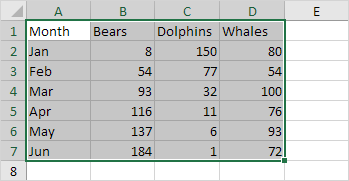
\includegraphics[width=0.6\linewidth]{pictures/Chart-SelectRange} \end{center}
\end{frame}

\begin{frame}[fragile]{Excel Charts And Graphs}
\protect\hypertarget{excel-charts-and-graphs-3}{}
To create a chart in Excel:

\begin{enumerate}
\setcounter{enumi}{1}
\tightlist
\item
  Click on the \texttt{‘Insert’} tab in the Excel toolbar and choose
  desired chart type.
\end{enumerate}

\begin{center}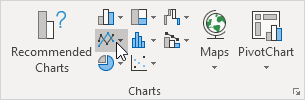
\includegraphics[width=0.45\linewidth,height=0.3\textheight]{pictures/Chart-Insert1} 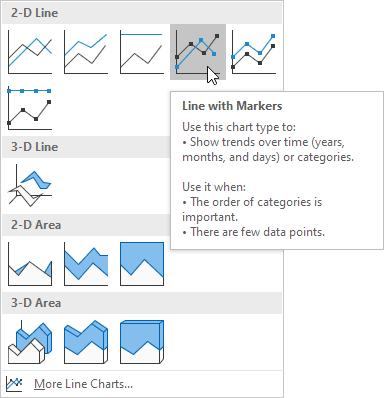
\includegraphics[width=0.45\linewidth,height=0.3\textheight]{pictures/Chart-Insert2} \end{center}
\end{frame}

\begin{frame}{Excel Charts And Graphs}
\protect\hypertarget{excel-charts-and-graphs-4}{}
To create a chart in Excel:

\begin{enumerate}
\setcounter{enumi}{2}
\tightlist
\item
  Customize your chart's design, layout, and formatting to meet your
  requirements.
\end{enumerate}

\begin{center}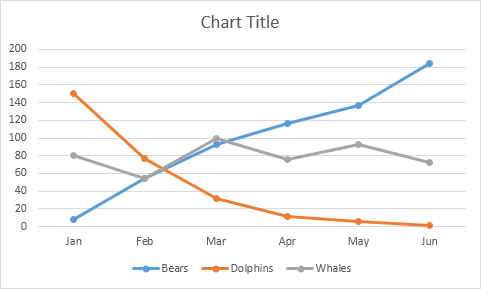
\includegraphics[width=0.6\linewidth]{pictures/Chart-Result} \end{center}
\end{frame}

\hypertarget{exercise-1.-data-on-a-single-variable.}{%
\section{Exercise 1. Data on a single
variable.}\label{exercise-1.-data-on-a-single-variable.}}

\begin{frame}{Exercise 1. Data on a single variable.}
\begin{itemize}
\item
  Data set: \texttt{ages.xlsx}
\item
  The (imaginary) ages of survey respondents, \(n = 30\).
\end{itemize}
\end{frame}

\begin{frame}{Part 1. Summary statistics.}
\protect\hypertarget{part-1.-summary-statistics.}{}
\begin{enumerate}
\item
  Create a new tab on the spreadsheet.
\item
  Compute the mean, median, min, max of ages using Excel functions. Make
  a table.
\item
  Compute the mean age using only the following excel commands:
  \textcolor{red}{SUM()}, \textcolor{red}{COUNT()}.
\item
  Which one is higher, the mean or the median? What does this tell us
  about the shape of the distribution of the data?
\end{enumerate}
\end{frame}

\begin{frame}{Part 2. Plotting data.}
\protect\hypertarget{part-2.-plotting-data.}{}
\begin{enumerate}
\item
  Create a new tab on the spreadsheet with the data from the original
  tab.
\item
  Compute a frequency distribution table. Decide yourself the cutoff
  points.
\item
  Compute a corresponding cumulative distribution table.
\item
  Make a graph describing the frequency distribution. The title should
  be \emph{``Frequency distribution (histogram)''}.
\item
  Make a graph describing the cumulative frequency distribution. The
  title should be \emph{``Cumulative Frequency distribution (ogive)''}.
\end{enumerate}
\end{frame}

\begin{frame}{Part 2. Plotting data.}
\protect\hypertarget{part-2.-plotting-data.-1}{}
\begin{itemize}
\tightlist
\item
  Two bar charts describe \emph{frequency distribution} and
  \emph{cumulative frequency distribution}.
\end{itemize}

\begin{center}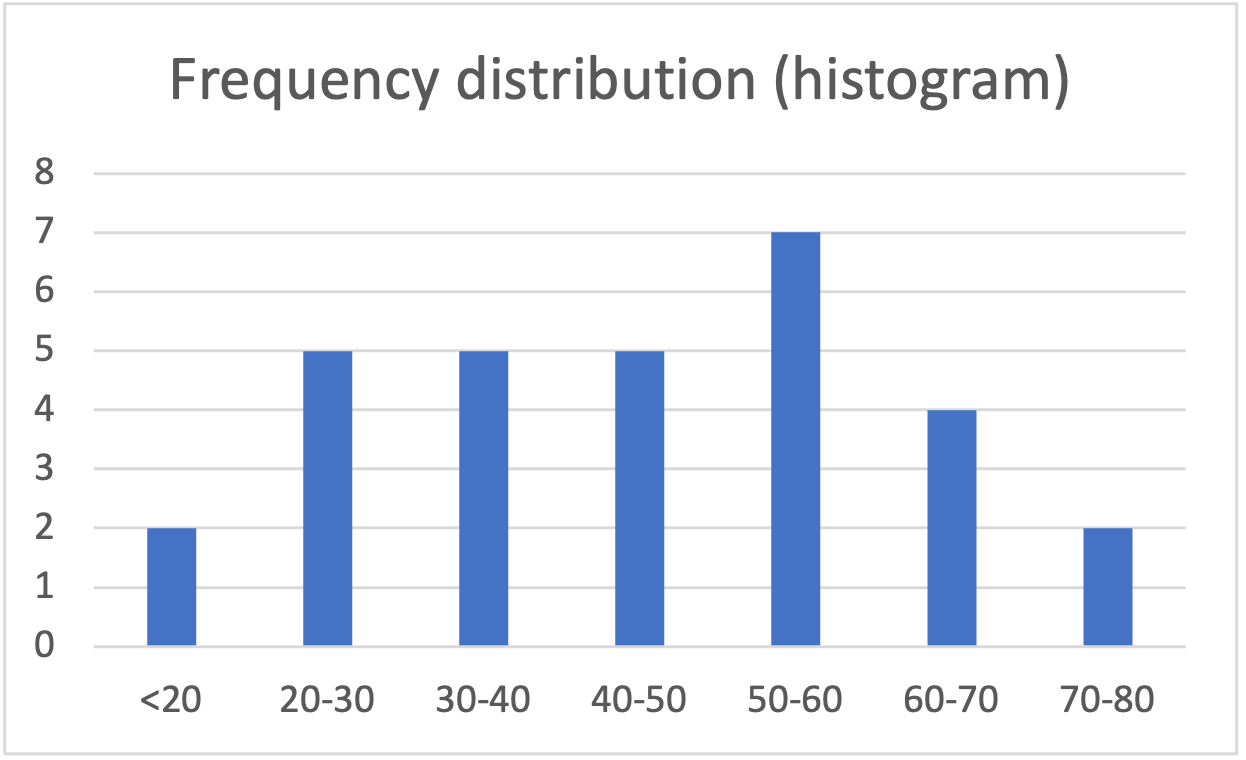
\includegraphics[width=0.45\linewidth,height=0.3\textheight]{pictures/Ex1-pmf-Histogram} 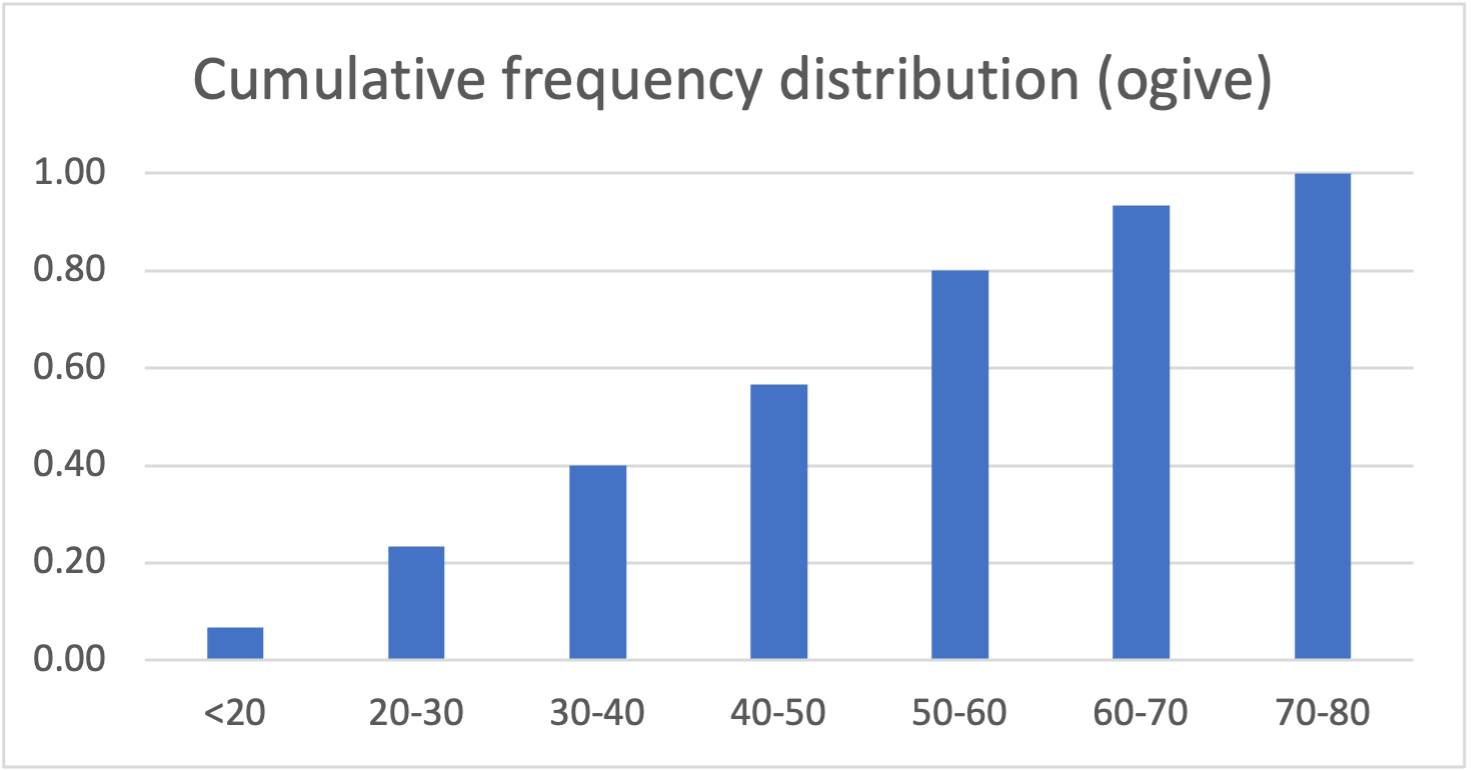
\includegraphics[width=0.45\linewidth,height=0.3\textheight]{pictures/Ex1-cdf-Ogive} \end{center}
\end{frame}

\begin{frame}{Part 3. Plotting data: Pie charts.}
\protect\hypertarget{part-3.-plotting-data-pie-charts.}{}
\begin{itemize}
\tightlist
\item
  A pie chart summarizes the age distribution.
\end{itemize}

\begin{center}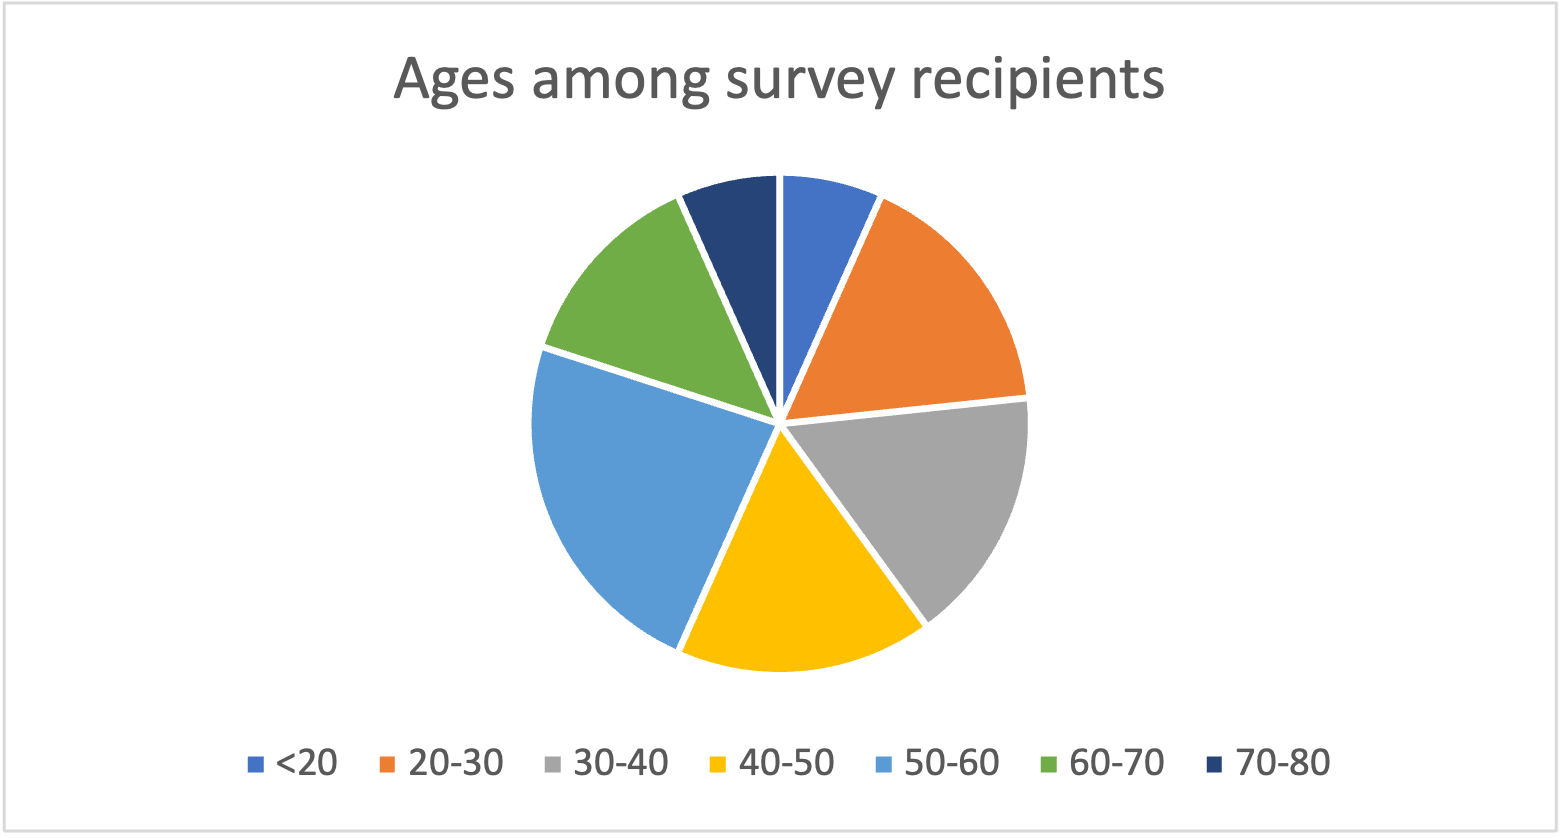
\includegraphics[width=0.6\linewidth]{pictures/Ex1-PieChart} \end{center}

\begin{itemize}
\tightlist
\item
  It emphasises the proportions of frequencies in each age group.
\end{itemize}
\end{frame}

\hypertarget{exercise-2.-data-on-multiple-variables.}{%
\section{Exercise 2. Data on multiple
variables.}\label{exercise-2.-data-on-multiple-variables.}}

\begin{frame}[fragile]{Exercise 2. Data on multiple variables.}
\begin{itemize}
\tightlist
\item
  Data set: \texttt{incomes.xlsx}
\item
  About (imaginary) data on two variables

  \begin{itemize}
  \tightlist
  \item
    income (\texttt{inc}), and
  \item
    years of schooling (\texttt{educ}), which is categorical and coded
    as follows:
  \end{itemize}
\end{itemize}

\begin{table}
\centering
\begin{tabular}[t]{ll}
\toprule
 & \\
\midrule
9 & Grade 9\\
10 & Grade 10\\
11 & Grade 11\\
12 & Grade 12\\
13 & 1 year of college\\
... & \\
17 & 5 years of college\\
18 & 6+ years of college\\
\bottomrule
\end{tabular}
\end{table}
\end{frame}

\begin{frame}{Part 1. Correlation}
\protect\hypertarget{part-1.-correlation}{}
\begin{itemize}
\tightlist
\item
  Open up the data and create a new tab with the original data.
\item
  Compute the sample mean and the sample variance of both variables.
\item
  Compute the coefficient of correlation between income and years of
  schooling. How do we interpret the correlation coefficient? Is it a
  large or a small coefficient?
\end{itemize}
\end{frame}

\begin{frame}{Part 1. Correlation}
\protect\hypertarget{part-1.-correlation-1}{}
\begin{itemize}
\item
  Coefficient of Correlation summarises the \emph{direction} and
  \emph{strength} of the linear relationship between two quantitative
  variables.
\item
  Sample correlation coefficient \[
  r = \frac{s_{xy}}{s_x s_y}
  \]
\item
  \textbf{Magnitude of correlation}\\
  Often, when we discuss correlations, we use the following rules of
  thumb:

  \begin{itemize}
  \tightlist
  \item
    \(\mid r \mid < 0.2\): small correlation
  \item
    \(0.2 \leq \mid r \mid \leq 0.8\): medium correlation
  \item
    \(\mid r \mid > 0.8\): very strong correlation
  \end{itemize}
\end{itemize}
\end{frame}

\begin{frame}{Part 2. Scatterplots}
\protect\hypertarget{part-2.-scatterplots}{}
\begin{itemize}
\tightlist
\item
  Create a new tab with the original data.
\item
  Make a scatterplot of the data. This is a plot where each individual
  (each row in the data) is described as a dot, and the x-axis value
  shows the years of education, the y-axis value shows the income of the
  individual.
\item
  How does the scatterplot reflect the correlation coefficient from Part
  1?
\end{itemize}
\end{frame}

\begin{frame}{Part 2. Scatterplots}
\protect\hypertarget{part-2.-scatterplots-1}{}
\begin{itemize}
\tightlist
\item
  A scatterplot of the data where each individual (each row in the data)
  is described as a dot, and the x-axis value shows the years of
  education, the y-axis value shows the income of the individual.
\end{itemize}

\begin{center}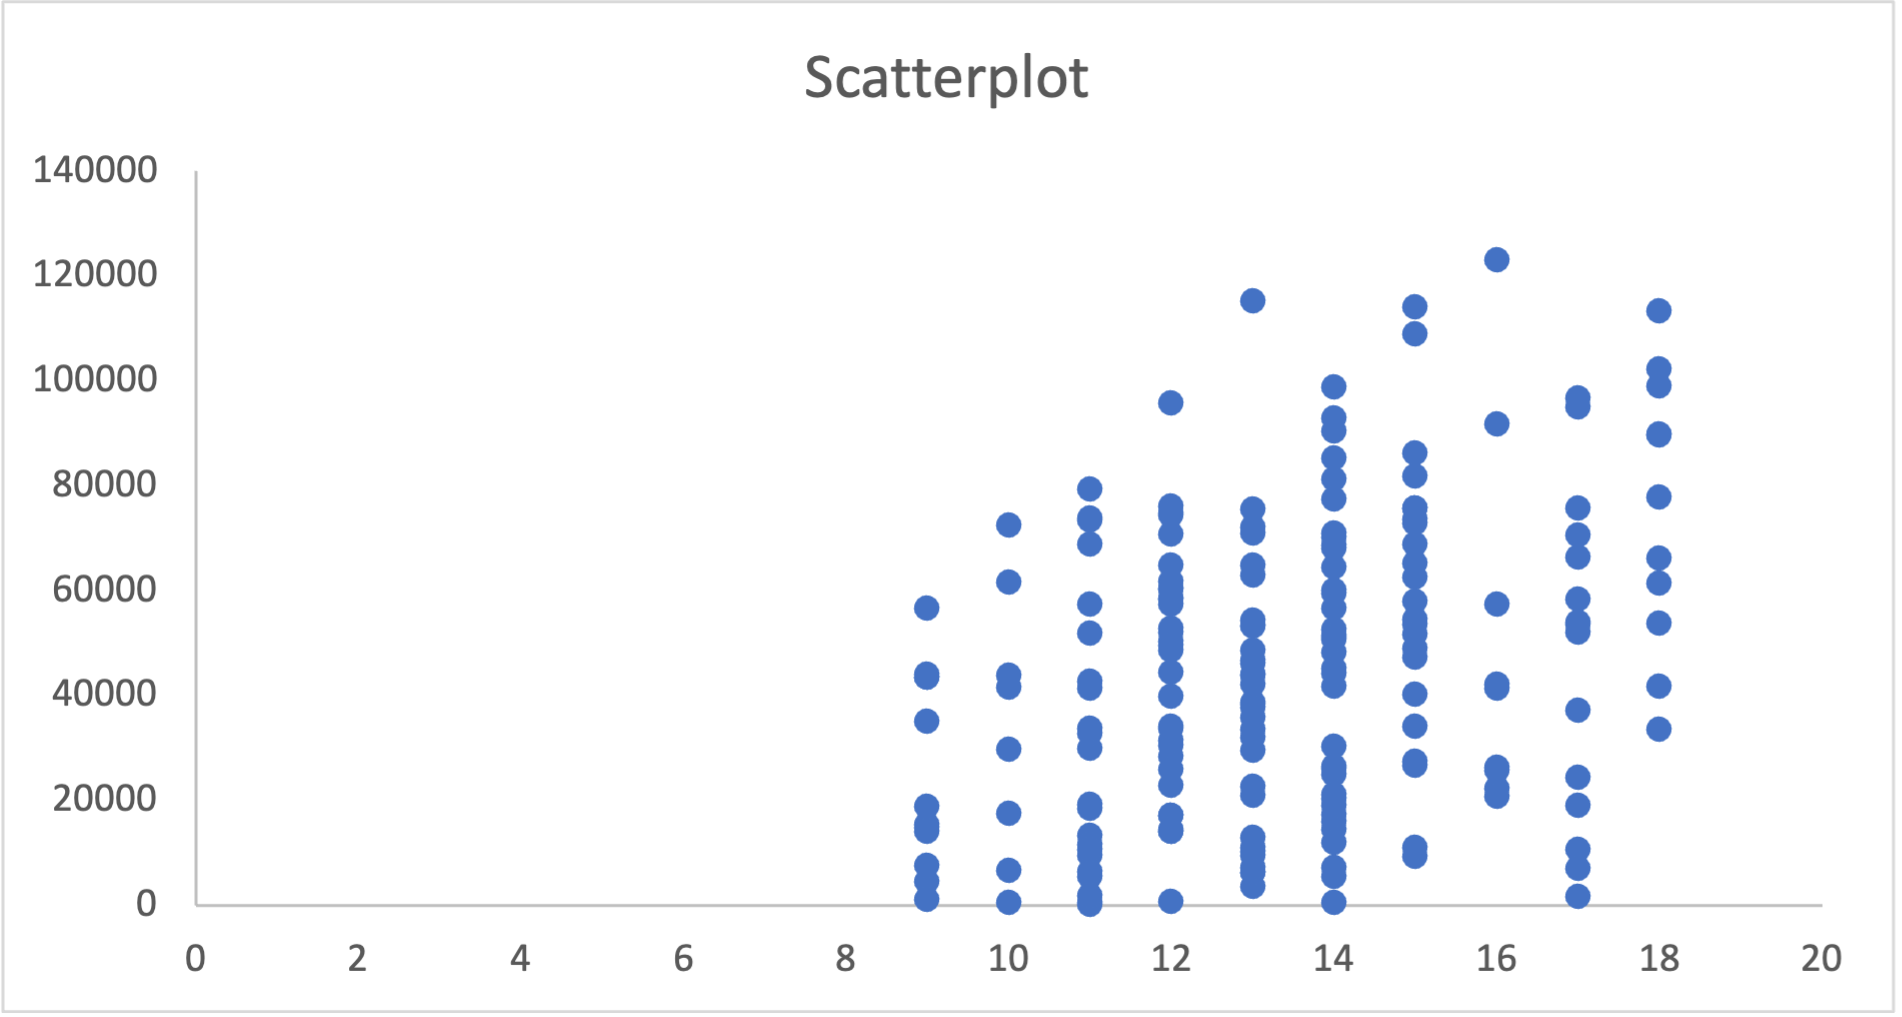
\includegraphics[width=0.6\linewidth]{pictures/Ex2-ScatterPlot} \end{center}
\end{frame}

\begin{frame}{Part 3. Binned plots}
\protect\hypertarget{part-3.-binned-plots}{}
\begin{itemize}
\tightlist
\item
  The scatterplot can be hard to read when there are many observations.
  Different data visualization tools can make the data easier to
  interpret.
\item
  Create a new tab with the original data.
\item
  For each value of ``educ'', compute the conditional average of income.
  That means that for each level of education you calculate the average
  income\\
  (Hint: Use Excel formulas \textcolor{red}{UNIQUE()} and
  \textcolor{red}{AVERAGEIF()}).
\item
  Make a binned plot where x-axis is the years of education and y-axis
  is the average income for the given level of education.\\
  (Hint: There will be only one dot in the picture for each years of
  schooling).
\item
  When can a binned plot be more informative than a scatterplot?
\end{itemize}
\end{frame}

\begin{frame}{Part 3. Binned plots}
\protect\hypertarget{part-3.-binned-plots-1}{}
\begin{itemize}
\tightlist
\item
  A binned plot where x-axis is the years of education and y-axis is the
  average income for the given level of education.
\end{itemize}

\begin{center}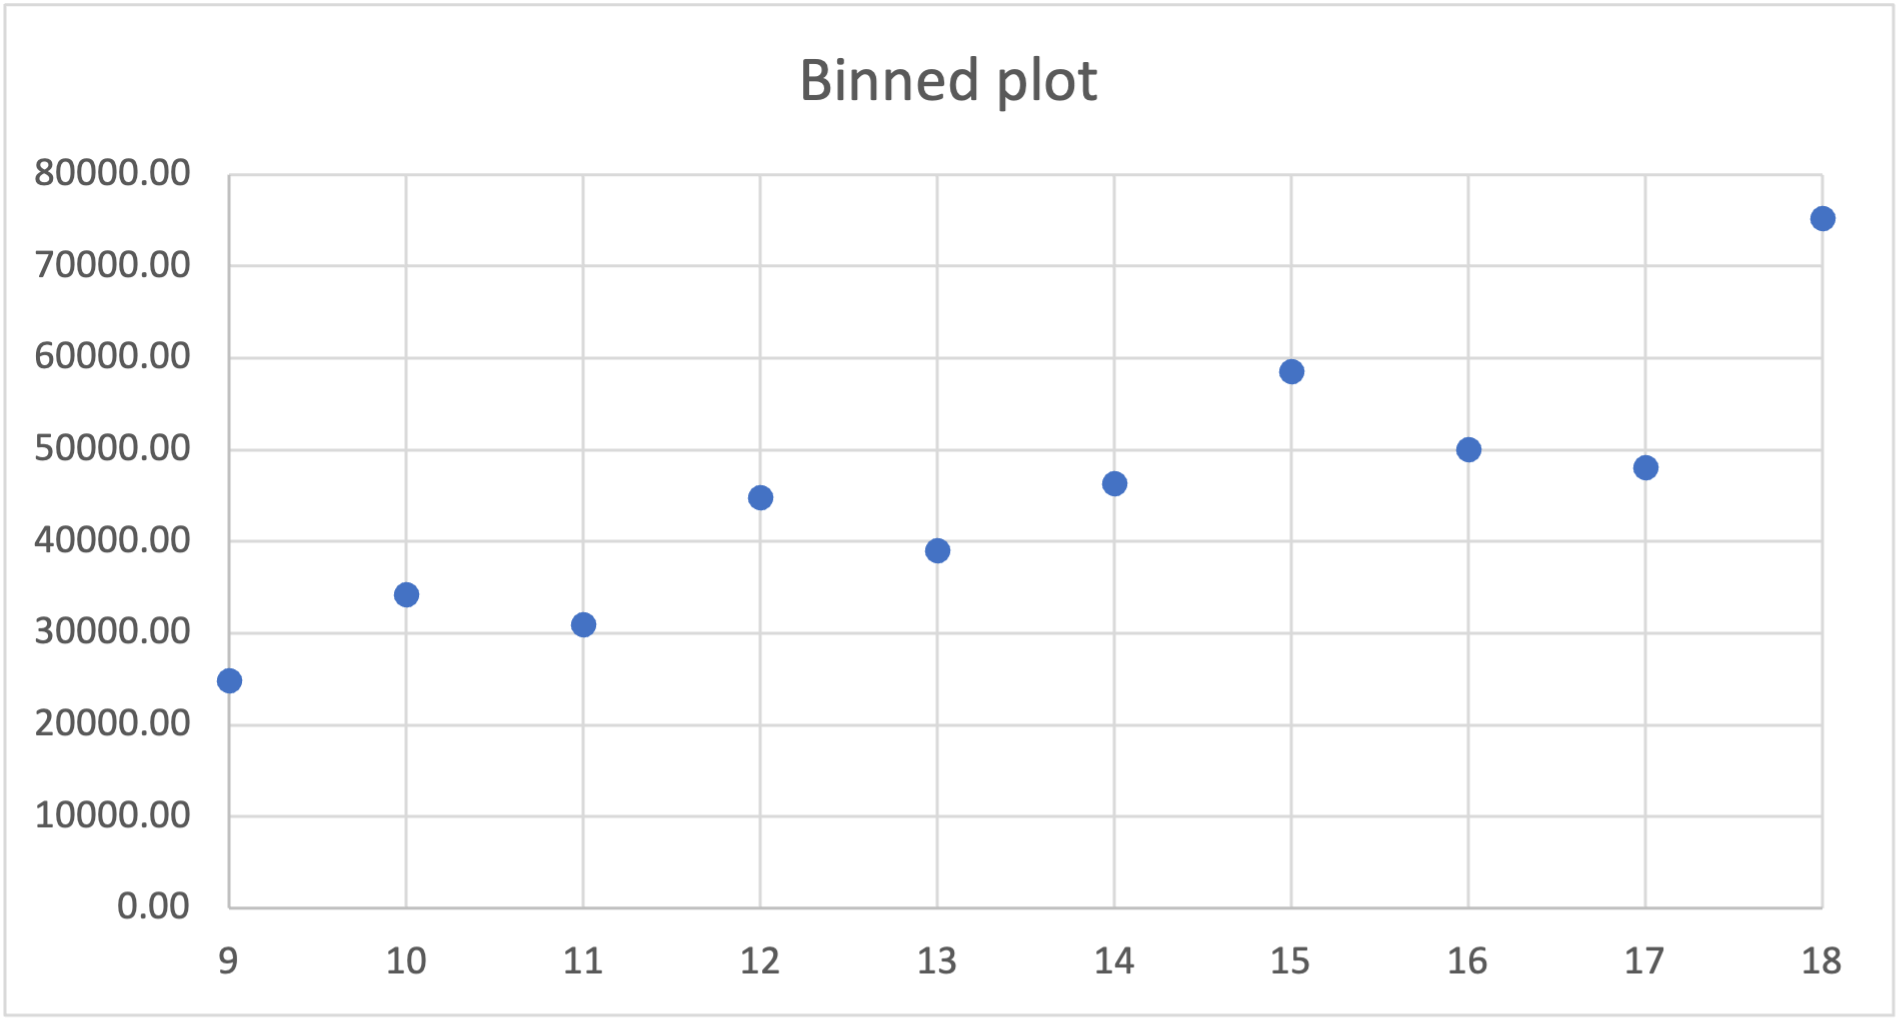
\includegraphics[width=0.6\linewidth]{pictures/Ex2-BinnedPlot} \end{center}

\begin{itemize}
\tightlist
\item
  There will be only one dot in the picture for each years of schooling.
\end{itemize}
\end{frame}

\begin{frame}{Part 3. Binned plots}
\protect\hypertarget{part-3.-binned-plots-2}{}
\begin{itemize}
\tightlist
\item
  A binned plot is often used when we want to describe the association
  (correlation) between two variables, but there are too many
  observations to make an informative scatterplot.
\end{itemize}
\end{frame}

\begin{frame}{Part 4 {[}opt{]}. Percentiles and IF-statements on Excel}
\protect\hypertarget{part-4-opt.-percentiles-and-if-statements-on-excel}{}
\begin{itemize}
\tightlist
\item
  Compute the \(50^{\text{th}}\) percentile of the data (the median)
  conditional on years of education.\\
  (Hint: you should calculate the \(50^{\text{th}}\) percentile for all
  values of years of education; use formula
  \textcolor{red}{MEDIAN(IF())})
\item
  Compute the \(25^{\text{th}}\) and the \(75^{\text{th}}\) percentiles
  of the data conditional on years of education.\\
  (Hint: use formula \textcolor{red}{PERCENTILE(IF())})
\item
  How do we interpret the table?
\end{itemize}
\end{frame}

\begin{frame}{REFERENCES}
\protect\hypertarget{references}{}
\begin{enumerate}
\item
  Excel Cheetsheet:\\
  \url{https://blog.enterprisedna.co/excel-cheat-sheet/}
\item
  Create charts in Excel:\\
  \url{https://www.excel-easy.com/data-analysis/charts.html\#google_vignette}
\end{enumerate}
\end{frame}

\end{document}
